
% Default to the notebook output style




% Inherit from the specified cell style.





\documentclass[11pt]{article}



    \usepackage[T1]{fontenc}
    % Nicer default font (+ math font) than Computer Modern for most use cases
    \usepackage{mathpazo}

    % Basic figure setup, for now with no caption control since it's done
    % automatically by Pandoc (which extracts ![](path) syntax from Markdown).
    \usepackage{graphicx}
    % We will generate all images so they have a width \maxwidth. This means
    % that they will get their normal width if they fit onto the page, but
    % are scaled down if they would overflow the margins.
    \makeatletter
    \def\maxwidth{\ifdim\Gin@nat@width>\linewidth\linewidth
    \else\Gin@nat@width\fi}
    \makeatother
    \let\Oldincludegraphics\includegraphics
    % Set max figure width to be 80% of text width, for now hardcoded.
    \renewcommand{\includegraphics}[1]{\Oldincludegraphics[width=.8\maxwidth]{#1}}
    % Ensure that by default, figures have no caption (until we provide a
    % proper Figure object with a Caption API and a way to capture that
    % in the conversion process - todo).
    \usepackage{caption}
    \DeclareCaptionLabelFormat{nolabel}{}
    \captionsetup{labelformat=nolabel}

    \usepackage{adjustbox} % Used to constrain images to a maximum size
    \usepackage{xcolor} % Allow colors to be defined
    \usepackage{enumerate} % Needed for markdown enumerations to work
    \usepackage{geometry} % Used to adjust the document margins
    \usepackage{amsmath} % Equations
    \usepackage{amssymb} % Equations
    \usepackage{textcomp} % defines textquotesingle
    % Hack from http://tex.stackexchange.com/a/47451/13684:
    \AtBeginDocument{%
        \def\PYZsq{\textquotesingle}% Upright quotes in Pygmentized code
    }
    \usepackage{upquote} % Upright quotes for verbatim code
    \usepackage{eurosym} % defines \euro
    \usepackage[mathletters]{ucs} % Extended unicode (utf-8) support
    \usepackage[utf8x]{inputenc} % Allow utf-8 characters in the tex document
    \usepackage{fancyvrb} % verbatim replacement that allows latex
    \usepackage{grffile} % extends the file name processing of package graphics
                         % to support a larger range
    % The hyperref package gives us a pdf with properly built
    % internal navigation ('pdf bookmarks' for the table of contents,
    % internal cross-reference links, web links for URLs, etc.)
    \usepackage{hyperref}
    \usepackage{longtable} % longtable support required by pandoc >1.10
    \usepackage{booktabs}  % table support for pandoc > 1.12.2
    \usepackage[inline]{enumitem} % IRkernel/repr support (it uses the enumerate* environment)
    \usepackage[normalem]{ulem} % ulem is needed to support strikethroughs (\sout)
                                % normalem makes italics be italics, not underlines




    % Colors for the hyperref package
    \definecolor{urlcolor}{rgb}{0,.145,.698}
    \definecolor{linkcolor}{rgb}{.71,0.21,0.01}
    \definecolor{citecolor}{rgb}{.12,.54,.11}

    % ANSI colors
    \definecolor{ansi-black}{HTML}{3E424D}
    \definecolor{ansi-black-intense}{HTML}{282C36}
    \definecolor{ansi-red}{HTML}{E75C58}
    \definecolor{ansi-red-intense}{HTML}{B22B31}
    \definecolor{ansi-green}{HTML}{00A250}
    \definecolor{ansi-green-intense}{HTML}{007427}
    \definecolor{ansi-yellow}{HTML}{DDB62B}
    \definecolor{ansi-yellow-intense}{HTML}{B27D12}
    \definecolor{ansi-blue}{HTML}{208FFB}
    \definecolor{ansi-blue-intense}{HTML}{0065CA}
    \definecolor{ansi-magenta}{HTML}{D160C4}
    \definecolor{ansi-magenta-intense}{HTML}{A03196}
    \definecolor{ansi-cyan}{HTML}{60C6C8}
    \definecolor{ansi-cyan-intense}{HTML}{258F8F}
    \definecolor{ansi-white}{HTML}{C5C1B4}
    \definecolor{ansi-white-intense}{HTML}{A1A6B2}

    % commands and environments needed by pandoc snippets
    % extracted from the output of `pandoc -s`
    \providecommand{\tightlist}{%
      \setlength{\itemsep}{0pt}\setlength{\parskip}{0pt}}
    \DefineVerbatimEnvironment{Highlighting}{Verbatim}{commandchars=\\\{\}}
    % Add ',fontsize=\small' for more characters per line
    \newenvironment{Shaded}{}{}
    \newcommand{\KeywordTok}[1]{\textcolor[rgb]{0.00,0.44,0.13}{\textbf{{#1}}}}
    \newcommand{\DataTypeTok}[1]{\textcolor[rgb]{0.56,0.13,0.00}{{#1}}}
    \newcommand{\DecValTok}[1]{\textcolor[rgb]{0.25,0.63,0.44}{{#1}}}
    \newcommand{\BaseNTok}[1]{\textcolor[rgb]{0.25,0.63,0.44}{{#1}}}
    \newcommand{\FloatTok}[1]{\textcolor[rgb]{0.25,0.63,0.44}{{#1}}}
    \newcommand{\CharTok}[1]{\textcolor[rgb]{0.25,0.44,0.63}{{#1}}}
    \newcommand{\StringTok}[1]{\textcolor[rgb]{0.25,0.44,0.63}{{#1}}}
    \newcommand{\CommentTok}[1]{\textcolor[rgb]{0.38,0.63,0.69}{\textit{{#1}}}}
    \newcommand{\OtherTok}[1]{\textcolor[rgb]{0.00,0.44,0.13}{{#1}}}
    \newcommand{\AlertTok}[1]{\textcolor[rgb]{1.00,0.00,0.00}{\textbf{{#1}}}}
    \newcommand{\FunctionTok}[1]{\textcolor[rgb]{0.02,0.16,0.49}{{#1}}}
    \newcommand{\RegionMarkerTok}[1]{{#1}}
    \newcommand{\ErrorTok}[1]{\textcolor[rgb]{1.00,0.00,0.00}{\textbf{{#1}}}}
    \newcommand{\NormalTok}[1]{{#1}}

    % Additional commands for more recent versions of Pandoc
    \newcommand{\ConstantTok}[1]{\textcolor[rgb]{0.53,0.00,0.00}{{#1}}}
    \newcommand{\SpecialCharTok}[1]{\textcolor[rgb]{0.25,0.44,0.63}{{#1}}}
    \newcommand{\VerbatimStringTok}[1]{\textcolor[rgb]{0.25,0.44,0.63}{{#1}}}
    \newcommand{\SpecialStringTok}[1]{\textcolor[rgb]{0.73,0.40,0.53}{{#1}}}
    \newcommand{\ImportTok}[1]{{#1}}
    \newcommand{\DocumentationTok}[1]{\textcolor[rgb]{0.73,0.13,0.13}{\textit{{#1}}}}
    \newcommand{\AnnotationTok}[1]{\textcolor[rgb]{0.38,0.63,0.69}{\textbf{\textit{{#1}}}}}
    \newcommand{\CommentVarTok}[1]{\textcolor[rgb]{0.38,0.63,0.69}{\textbf{\textit{{#1}}}}}
    \newcommand{\VariableTok}[1]{\textcolor[rgb]{0.10,0.09,0.49}{{#1}}}
    \newcommand{\ControlFlowTok}[1]{\textcolor[rgb]{0.00,0.44,0.13}{\textbf{{#1}}}}
    \newcommand{\OperatorTok}[1]{\textcolor[rgb]{0.40,0.40,0.40}{{#1}}}
    \newcommand{\BuiltInTok}[1]{{#1}}
    \newcommand{\ExtensionTok}[1]{{#1}}
    \newcommand{\PreprocessorTok}[1]{\textcolor[rgb]{0.74,0.48,0.00}{{#1}}}
    \newcommand{\AttributeTok}[1]{\textcolor[rgb]{0.49,0.56,0.16}{{#1}}}
    \newcommand{\InformationTok}[1]{\textcolor[rgb]{0.38,0.63,0.69}{\textbf{\textit{{#1}}}}}
    \newcommand{\WarningTok}[1]{\textcolor[rgb]{0.38,0.63,0.69}{\textbf{\textit{{#1}}}}}


\newenvironment{figurehere}
  {\def\@captype{figure}}
  {}
\makeatother

    % Define a nice break command that doesn't care if a line doesn't already
    % exist.
    \def\br{\hspace*{\fill} \\* }
    % Math Jax compatability definitions
    \def\gt{>}
    \def\lt{<}
    % Document parameters
    \title{Lista1\_IOF814}




    % Pygments definitions

\makeatletter
\def\PY@reset{\let\PY@it=\relax \let\PY@bf=\relax%
    \let\PY@ul=\relax \let\PY@tc=\relax%
    \let\PY@bc=\relax \let\PY@ff=\relax}
\def\PY@tok#1{\csname PY@tok@#1\endcsname}
\def\PY@toks#1+{\ifx\relax#1\empty\else%
    \PY@tok{#1}\expandafter\PY@toks\fi}
\def\PY@do#1{\PY@bc{\PY@tc{\PY@ul{%
    \PY@it{\PY@bf{\PY@ff{#1}}}}}}}
\def\PY#1#2{\PY@reset\PY@toks#1+\relax+\PY@do{#2}}

\expandafter\def\csname PY@tok@gd\endcsname{\def\PY@tc##1{\textcolor[rgb]{0.63,0.00,0.00}{##1}}}
\expandafter\def\csname PY@tok@gu\endcsname{\let\PY@bf=\textbf\def\PY@tc##1{\textcolor[rgb]{0.50,0.00,0.50}{##1}}}
\expandafter\def\csname PY@tok@gt\endcsname{\def\PY@tc##1{\textcolor[rgb]{0.00,0.27,0.87}{##1}}}
\expandafter\def\csname PY@tok@gs\endcsname{\let\PY@bf=\textbf}
\expandafter\def\csname PY@tok@gr\endcsname{\def\PY@tc##1{\textcolor[rgb]{1.00,0.00,0.00}{##1}}}
\expandafter\def\csname PY@tok@cm\endcsname{\let\PY@it=\textit\def\PY@tc##1{\textcolor[rgb]{0.25,0.50,0.50}{##1}}}
\expandafter\def\csname PY@tok@vg\endcsname{\def\PY@tc##1{\textcolor[rgb]{0.10,0.09,0.49}{##1}}}
\expandafter\def\csname PY@tok@vi\endcsname{\def\PY@tc##1{\textcolor[rgb]{0.10,0.09,0.49}{##1}}}
\expandafter\def\csname PY@tok@mh\endcsname{\def\PY@tc##1{\textcolor[rgb]{0.40,0.40,0.40}{##1}}}
\expandafter\def\csname PY@tok@cs\endcsname{\let\PY@it=\textit\def\PY@tc##1{\textcolor[rgb]{0.25,0.50,0.50}{##1}}}
\expandafter\def\csname PY@tok@ge\endcsname{\let\PY@it=\textit}
\expandafter\def\csname PY@tok@vc\endcsname{\def\PY@tc##1{\textcolor[rgb]{0.10,0.09,0.49}{##1}}}
\expandafter\def\csname PY@tok@il\endcsname{\def\PY@tc##1{\textcolor[rgb]{0.40,0.40,0.40}{##1}}}
\expandafter\def\csname PY@tok@go\endcsname{\def\PY@tc##1{\textcolor[rgb]{0.53,0.53,0.53}{##1}}}
\expandafter\def\csname PY@tok@cp\endcsname{\def\PY@tc##1{\textcolor[rgb]{0.74,0.48,0.00}{##1}}}
\expandafter\def\csname PY@tok@gi\endcsname{\def\PY@tc##1{\textcolor[rgb]{0.00,0.63,0.00}{##1}}}
\expandafter\def\csname PY@tok@gh\endcsname{\let\PY@bf=\textbf\def\PY@tc##1{\textcolor[rgb]{0.00,0.00,0.50}{##1}}}
\expandafter\def\csname PY@tok@ni\endcsname{\let\PY@bf=\textbf\def\PY@tc##1{\textcolor[rgb]{0.60,0.60,0.60}{##1}}}
\expandafter\def\csname PY@tok@nl\endcsname{\def\PY@tc##1{\textcolor[rgb]{0.63,0.63,0.00}{##1}}}
\expandafter\def\csname PY@tok@nn\endcsname{\let\PY@bf=\textbf\def\PY@tc##1{\textcolor[rgb]{0.00,0.00,1.00}{##1}}}
\expandafter\def\csname PY@tok@no\endcsname{\def\PY@tc##1{\textcolor[rgb]{0.53,0.00,0.00}{##1}}}
\expandafter\def\csname PY@tok@na\endcsname{\def\PY@tc##1{\textcolor[rgb]{0.49,0.56,0.16}{##1}}}
\expandafter\def\csname PY@tok@nb\endcsname{\def\PY@tc##1{\textcolor[rgb]{0.00,0.50,0.00}{##1}}}
\expandafter\def\csname PY@tok@nc\endcsname{\let\PY@bf=\textbf\def\PY@tc##1{\textcolor[rgb]{0.00,0.00,1.00}{##1}}}
\expandafter\def\csname PY@tok@nd\endcsname{\def\PY@tc##1{\textcolor[rgb]{0.67,0.13,1.00}{##1}}}
\expandafter\def\csname PY@tok@ne\endcsname{\let\PY@bf=\textbf\def\PY@tc##1{\textcolor[rgb]{0.82,0.25,0.23}{##1}}}
\expandafter\def\csname PY@tok@nf\endcsname{\def\PY@tc##1{\textcolor[rgb]{0.00,0.00,1.00}{##1}}}
\expandafter\def\csname PY@tok@si\endcsname{\let\PY@bf=\textbf\def\PY@tc##1{\textcolor[rgb]{0.73,0.40,0.53}{##1}}}
\expandafter\def\csname PY@tok@s2\endcsname{\def\PY@tc##1{\textcolor[rgb]{0.73,0.13,0.13}{##1}}}
\expandafter\def\csname PY@tok@nt\endcsname{\let\PY@bf=\textbf\def\PY@tc##1{\textcolor[rgb]{0.00,0.50,0.00}{##1}}}
\expandafter\def\csname PY@tok@nv\endcsname{\def\PY@tc##1{\textcolor[rgb]{0.10,0.09,0.49}{##1}}}
\expandafter\def\csname PY@tok@s1\endcsname{\def\PY@tc##1{\textcolor[rgb]{0.73,0.13,0.13}{##1}}}
\expandafter\def\csname PY@tok@ch\endcsname{\let\PY@it=\textit\def\PY@tc##1{\textcolor[rgb]{0.25,0.50,0.50}{##1}}}
\expandafter\def\csname PY@tok@m\endcsname{\def\PY@tc##1{\textcolor[rgb]{0.40,0.40,0.40}{##1}}}
\expandafter\def\csname PY@tok@gp\endcsname{\let\PY@bf=\textbf\def\PY@tc##1{\textcolor[rgb]{0.00,0.00,0.50}{##1}}}
\expandafter\def\csname PY@tok@sh\endcsname{\def\PY@tc##1{\textcolor[rgb]{0.73,0.13,0.13}{##1}}}
\expandafter\def\csname PY@tok@ow\endcsname{\let\PY@bf=\textbf\def\PY@tc##1{\textcolor[rgb]{0.67,0.13,1.00}{##1}}}
\expandafter\def\csname PY@tok@sx\endcsname{\def\PY@tc##1{\textcolor[rgb]{0.00,0.50,0.00}{##1}}}
\expandafter\def\csname PY@tok@bp\endcsname{\def\PY@tc##1{\textcolor[rgb]{0.00,0.50,0.00}{##1}}}
\expandafter\def\csname PY@tok@c1\endcsname{\let\PY@it=\textit\def\PY@tc##1{\textcolor[rgb]{0.25,0.50,0.50}{##1}}}
\expandafter\def\csname PY@tok@o\endcsname{\def\PY@tc##1{\textcolor[rgb]{0.40,0.40,0.40}{##1}}}
\expandafter\def\csname PY@tok@kc\endcsname{\let\PY@bf=\textbf\def\PY@tc##1{\textcolor[rgb]{0.00,0.50,0.00}{##1}}}
\expandafter\def\csname PY@tok@c\endcsname{\let\PY@it=\textit\def\PY@tc##1{\textcolor[rgb]{0.25,0.50,0.50}{##1}}}
\expandafter\def\csname PY@tok@mf\endcsname{\def\PY@tc##1{\textcolor[rgb]{0.40,0.40,0.40}{##1}}}
\expandafter\def\csname PY@tok@err\endcsname{\def\PY@bc##1{\setlength{\fboxsep}{0pt}\fcolorbox[rgb]{1.00,0.00,0.00}{1,1,1}{\strut ##1}}}
\expandafter\def\csname PY@tok@mb\endcsname{\def\PY@tc##1{\textcolor[rgb]{0.40,0.40,0.40}{##1}}}
\expandafter\def\csname PY@tok@ss\endcsname{\def\PY@tc##1{\textcolor[rgb]{0.10,0.09,0.49}{##1}}}
\expandafter\def\csname PY@tok@sr\endcsname{\def\PY@tc##1{\textcolor[rgb]{0.73,0.40,0.53}{##1}}}
\expandafter\def\csname PY@tok@mo\endcsname{\def\PY@tc##1{\textcolor[rgb]{0.40,0.40,0.40}{##1}}}
\expandafter\def\csname PY@tok@kd\endcsname{\let\PY@bf=\textbf\def\PY@tc##1{\textcolor[rgb]{0.00,0.50,0.00}{##1}}}
\expandafter\def\csname PY@tok@mi\endcsname{\def\PY@tc##1{\textcolor[rgb]{0.40,0.40,0.40}{##1}}}
\expandafter\def\csname PY@tok@kn\endcsname{\let\PY@bf=\textbf\def\PY@tc##1{\textcolor[rgb]{0.00,0.50,0.00}{##1}}}
\expandafter\def\csname PY@tok@cpf\endcsname{\let\PY@it=\textit\def\PY@tc##1{\textcolor[rgb]{0.25,0.50,0.50}{##1}}}
\expandafter\def\csname PY@tok@kr\endcsname{\let\PY@bf=\textbf\def\PY@tc##1{\textcolor[rgb]{0.00,0.50,0.00}{##1}}}
\expandafter\def\csname PY@tok@s\endcsname{\def\PY@tc##1{\textcolor[rgb]{0.73,0.13,0.13}{##1}}}
\expandafter\def\csname PY@tok@kp\endcsname{\def\PY@tc##1{\textcolor[rgb]{0.00,0.50,0.00}{##1}}}
\expandafter\def\csname PY@tok@w\endcsname{\def\PY@tc##1{\textcolor[rgb]{0.73,0.73,0.73}{##1}}}
\expandafter\def\csname PY@tok@kt\endcsname{\def\PY@tc##1{\textcolor[rgb]{0.69,0.00,0.25}{##1}}}
\expandafter\def\csname PY@tok@sc\endcsname{\def\PY@tc##1{\textcolor[rgb]{0.73,0.13,0.13}{##1}}}
\expandafter\def\csname PY@tok@sb\endcsname{\def\PY@tc##1{\textcolor[rgb]{0.73,0.13,0.13}{##1}}}
\expandafter\def\csname PY@tok@k\endcsname{\let\PY@bf=\textbf\def\PY@tc##1{\textcolor[rgb]{0.00,0.50,0.00}{##1}}}
\expandafter\def\csname PY@tok@se\endcsname{\let\PY@bf=\textbf\def\PY@tc##1{\textcolor[rgb]{0.73,0.40,0.13}{##1}}}
\expandafter\def\csname PY@tok@sd\endcsname{\let\PY@it=\textit\def\PY@tc##1{\textcolor[rgb]{0.73,0.13,0.13}{##1}}}

\def\PYZbs{\char`\\}
\def\PYZus{\char`\_}
\def\PYZob{\char`\{}
\def\PYZcb{\char`\}}
\def\PYZca{\char`\^}
\def\PYZam{\char`\&}
\def\PYZlt{\char`\<}
\def\PYZgt{\char`\>}
\def\PYZsh{\char`\#}
\def\PYZpc{\char`\%}
\def\PYZdl{\char`\$}
\def\PYZhy{\char`\-}
\def\PYZsq{\char`\'}
\def\PYZdq{\char`\"}
\def\PYZti{\char`\~}
% for compatibility with earlier versions
\def\PYZat{@}
\def\PYZlb{[}
\def\PYZrb{]}
\makeatother


    % Exact colors from NB
    \definecolor{incolor}{rgb}{0.0, 0.0, 0.5}
    \definecolor{outcolor}{rgb}{0.545, 0.0, 0.0}

    % Prevent overflowing lines due to hard-to-break entities
    \sloppy
    % Setup hyperref package
    \hypersetup{
      breaklinks=true,  % so long urls are correctly broken across lines
      colorlinks=true,
      urlcolor=urlcolor,
      linkcolor=linkcolor,
      citecolor=citecolor,
      }
    % Slightly bigger margins than the latex defaults

    \geometry{verbose,tmargin=1in,bmargin=1in,lmargin=1in,rmargin=1in}

\begin{document}


\title{Lista 1 - IOF814: Modelos Numéricos Aplicados a Processos Costeiros e Estuarinos}
\maketitle

\begin{center}
\textbf{Aluno:} Danilo Augusto Silva

\textbf{Nº USP:} 7279456

\textbf{Data de Entrega:} 31 de Outubro/2017
\end{center}
\vspace{0.5in}
Informações gerais quanto a estrutura da lista:

codes/: contem os códigos elaborados para os exercícios;

data/: contem os arquivos de input para alguns códigos e

outputs/: contem os arquivos de saída dos códigos, armazenados em
subpastas designada para cada questão, bem como o arquivo original \textbf{.tex}
e \textbf{.pdf} desta lista, com os desenvolvimentos das discretizações e
respostas dissertativas.

    \subparagraph{Q.01 - Demonstre que a solução da equação da difusão
unidimensional linear que utiliza esquema centrado no tempo e espaço é
incondicionalmente instável para uma solução explícita e
incondicionalmente estável para uma solução
implícita.}
A equação da difusão unidimensional linear é dada por:

\begin{equation}
\frac{\partial{f}}{\partial{x}} = D\frac{\partial^2{f}}{\partial{x^2}}
\label{ex1:1}
\end{equation}

onde \(D\) (\(D > 0\)) é o coeficiente de difusão.

Tomando a solução de (\ref{ex1:1}) de forma explícita, com esquema
centrado no espaço e no tempo, obtemos:

\begin{equation}
\frac{f^{n+1}_{j} - f^{n-1}_{j}}{2\Delta{t}} = \frac{D}{\Delta{x^2}}(f^{n}_{j+1} - 2f^{n}_{j} + f^{n}_{j-1})
\label{ex1:2}
\end{equation}

Ainda com (\ref{ex1:1}), podemos tomar a solução implícita com equema
centrado no espaço e no tempo, obtendo:

\begin{equation}
\frac{f^{n+1}_{j} - f^{n-1}_{j}}{2\Delta{t}} = \frac{D}{\Delta{x^2}}(f^{n+1}_{j+1} - 2f^{n+1}_{j} + f^{n+1}_{j-1})
\label{ex1:3}
\end{equation}

Para analisar a estabilidade das equações (\ref{ex1:2}) e (\ref{ex1:3}),
precisamos aplicar o Método de Von Neumann para estabilidade.

\textbf{Para a Eq. (2)}

Admitindo-se uma solução harmônica no espaço e polinomial no tempo, da
forma:

\begin{equation}
    f^{n}_{j} = B^{n}_{j}e^{iKj\Delta{x}}
    \label{ex1:4}
\end{equation}

onde \(K\) é o número de onda.

Aplicamos (\ref{ex1:4}) em (\ref{ex1:2}), obtendo:

\begin{equation}
    \frac{B^{n+1}e^{iKj\Delta{x}} - B^{n-1}e^{iKj\Delta{x}} }{2\Delta{x}} = \frac{D}{\Delta{x^2}}(B^{n}e^{iK(j+1)\Delta{x}} - 2B^{n}e^{iKj\Delta{x}} + B^{n}e^{iK(j-1)\Delta{x}})
    \label{ex1:5}
\end{equation}

A seguir, assumimos uma relação entre as amplitudes em instantes de
tempo sucessivos, onde:

\begin{equation}
    B^{n+1} = \lambda B^{n} e B^{n} = \lambda B^{n-1} \Rightarrow B^{n-1} = \lambda^{-1}B^n
    \label{ex1:6}
\end{equation}

Aplicando (\ref{ex1:6}) em (\ref{ex1:5}) e dividindo o resultado por
(\ref{ex1:4}), teremos:

\begin{equation}
    \frac{\lambda - \lambda^{-1}}{2\Delta{x}} = \frac{D}{\Delta{x^2}}(e^{iK\Delta{x}} - 2 + e^{-iK\Delta{x}})
    \label{ex1:7}
\end{equation}

Lembrando que \(e^{i\theta} = cos(\theta) - isin(\theta)\), então
(\ref{ex1:7}) é reescrita da seguinte forma:

\begin{equation}
    \frac{\lambda - \lambda^{-1}}{2\Delta{x}} = \frac{D}{\Delta{x^2}}(2cos(K\Delta{x}) - 2)
    \label{ex1:8}
\end{equation}

Desenvolvendo (\ref{ex1:8}) e considerando
\(q = 4\frac{\Delta{t}D}{\Delta{x^2}}\), temos:

\begin{equation}
    \lambda - \lambda^{-1} - q(cos(K\Delta{x} -1)) = 0
    \label{ex1:9}
\end{equation}

Manipulando (\ref{ex1:9}), chegamos em uma equação de 2º, da seguinte
forma:

\begin{equation}
    \lambda^{2} - \lambda q(cos(K\Delta{x} -1)) -1 = 0
    \label{ex1:10}
\end{equation}

A soluçao de (\ref{ex1:10}) é dada por:

\begin{equation}
    \lambda = \frac{qcos(K\Delta{x} -1) \pm \sqrt{q^2[cos(K\Delta{x})-1]^2 + 4} }{2}
    \label{ex1:11}
\end{equation}

Analisando (\ref{ex1:11}), nota-se que, para qualquer \(\Delta{x}\) e
\(\Delta{t}\), a solução de \(|\lambda| > 1\), ou seja, para qualquer
passo de tempo e de espaço a solução implícita com esquema centrado no
espaço e tempo será incondicionalmente instável.

\textbf{Para a Eq. (3)}

De forma análoga ao realizado para (2), fazemos para (3).

Aplicando (\ref{ex1:4}) em (\ref{ex1:3}):

\begin{equation}
        \frac{B^{n+1}e^{iKj\Delta{x}} - B^{n-1}e^{iKj\Delta{x}} }{2\Delta{x}} = \frac{D}{\Delta{x^2}}(B^{n+1}e^{iK(j+1)\Delta{x}} - 2B^{n+1}e^{iKj\Delta{x}} + B^{n+1}e^{iK(j-1)\Delta{x}})
        \label{ex1:12}
\end{equation}

Assumindo a relação (\ref{ex1:6}) e dividindo o resultado por
(\ref{ex1:4}), finalmente obtemos:

\begin{equation}
    \frac{\lambda - \lambda^{-1}}{2\Delta{x}} = \frac{D}{\Delta{x^2}}(\lambda e^{iK\Delta{x}} - 2\lambda + \lambda e^{-iK\Delta{x}})
    \label{ex1:13}
\end{equation}

Manipulando (\ref{ex1:13}), também chegamos em uma equação 2º:

\begin{equation}
    \lambda^{2}[1 - q(cos(K\Delta{x}) - 1)] = 1
    \label{ex1:14}
\end{equation}

Portando, a solução de (14) será:

\begin{equation}
    \lambda = \frac{1}{\sqrt{1 - q(cos(K\Delta{x}) - 1)}}
    \label{ex1:15}
\end{equation}

Analisando a equação (\ref{ex1:15}), nota-se que, para qualquer passo de
tempo e espaço, \(|\lambda| \le 1\) e, portanto, a solução implícita com
esquema centrado no tempo e espaço será incondionalmente estável.

    \begin{center}\rule{0.5\linewidth}{\linethickness}\end{center}

    \subparagraph{Q.02 - Implemente um modelo para a solução da equação da
advecção bi-dimensional por esquema semi-implícito centrado no tempo e
no
espaço.}

\begin{equation}
    \frac{\partial{f}}{\partial{t}} + u\frac{\partial{f}}{\partial{x}} + v\frac{\partial{f}}{\partial{y}} = 0
    \label{ex2:1}
\end{equation}

O esquema semi-implícito centrado no tempo e espaço é dado através da
média ponderada entre o esquema explícito e implícito, onde a soma do
peso deve ser 1. Desta forma, precisamos desenvolver ambos os esquemas,
para termos o requisitado no exercício.

\textbf{Esquema Explícito}

\begin{equation}
    \frac{ f^{n+1}_{j,k} - f^{n-1}_{j,k} }{2\Delta{x}} + u\frac{ f^{n}_{j+1,k} - f^{n}_{j-1,k} }{2\Delta{x}} + v\frac{f^{n}_{j,k+1} - f^{n}_{j,k-1}}{2\Delta{y}} = 0
    \label{ex2:2}
\end{equation}

\textbf{Esquema Implícito}

\begin{equation}
    \frac{ f^{n+1}_{j,k} - f^{n-1}_{j,k} }{2\Delta{x}} + u\frac{ f^{n+1}_{j+1,k} - f^{n+1}_{j-1,k} }{2\Delta{x}} + v\frac{f^{n+1}_{j,k+1} - f^{n+1}_{j,k-1}}{2\Delta{y}} = 0
    \label{ex2:3}
\end{equation}

A diferença entre (\ref{ex2:2}) e (\ref{ex2:3}) está no nível de tempo
utilizado para calcular as derivadas espaciais, respectivamente, n
(atual) e n+1 (renovado).

\textbf{Esquema Semi-Implícito}

\begin{equation}
    \frac{f^{n+1}_{j,k} - f^{n-1}_{j,k}}{2\Delta{t}} + \frac{u}{4\Delta{x}}(f^{n+1}_{j+1,k} - f^{n-1}_{j-1,k} + f^{n}_{j+1,k} - f^{n}_{j-1,k}) + \frac{v}{4\Delta{y}}( f^{n}_{j,k+1} - f^{n}_{j,k-1} + f^{n+1}_{j,k+1} -f^{n+1}_{j,k-1} ) = 0
    \label{ex2:4}
\end{equation}

Para resolver este problema numericamente, precisamos resolver um
sistema linear do tipo \(Ax=d\), onde A é uma matriz tri-diagonal, cuja
diagonal principal é preenchida com os coeficientes que multiplicam
todos os termos \(f^{n+1}\), o vetor d é composto por todos os termos
\(f^{n+1}\) e, por fim, x é o vetor de dados que queremos para o nível
renovado (n+1).

Desta forma, organizamos (\ref{ex2:4}) deixando os termos de instante
renovado do lado esquerdo e os demais termos do lado direito, como a
seguir:

\begin{equation}
\begin{multiline}
\begin{aligned}
    \frac{1}{2\Delta{t}}f^{n+1}_{j,k} + \frac{u}{4\Delta{x}}f^{n+1}_{j+1,k} - \frac{u}{4\Delta{x}}f^{n+1}_{j-1,k} + \frac{v}{4\Delta{y}}f^{n+1}_{j,k+1} - \frac{v}{4\Delta{y}}f^{n+1}_{j,k-1} =
    \frac{f^{n-1}_{j,k}}{2\Delta{t}} - \\
    \frac{u}{4\Delta{x}}f^{n}_{j+1,k} + \frac{u}{4\Delta{x}}f^{n}_{j-1,k} -
    \frac{v}{4\Delta{y}}f^{n}_{j,k+1} + \frac{v}{4\Delta{y}}f^{n}_{j,k-1}
    \label{ex2:5}
\end{aligned}
\end{multiline}
\end{equation}

A solução numérica de (\ref{ex2:5}) é apresentada no código
\textbf{lista1\_Q02} e algumas imagens podem ser observadas nas Fig~\ref{fig2:1}, Fig~\ref{fig2:2} e Fig~\ref{fig2:3}.


\begin{figure}
\centering
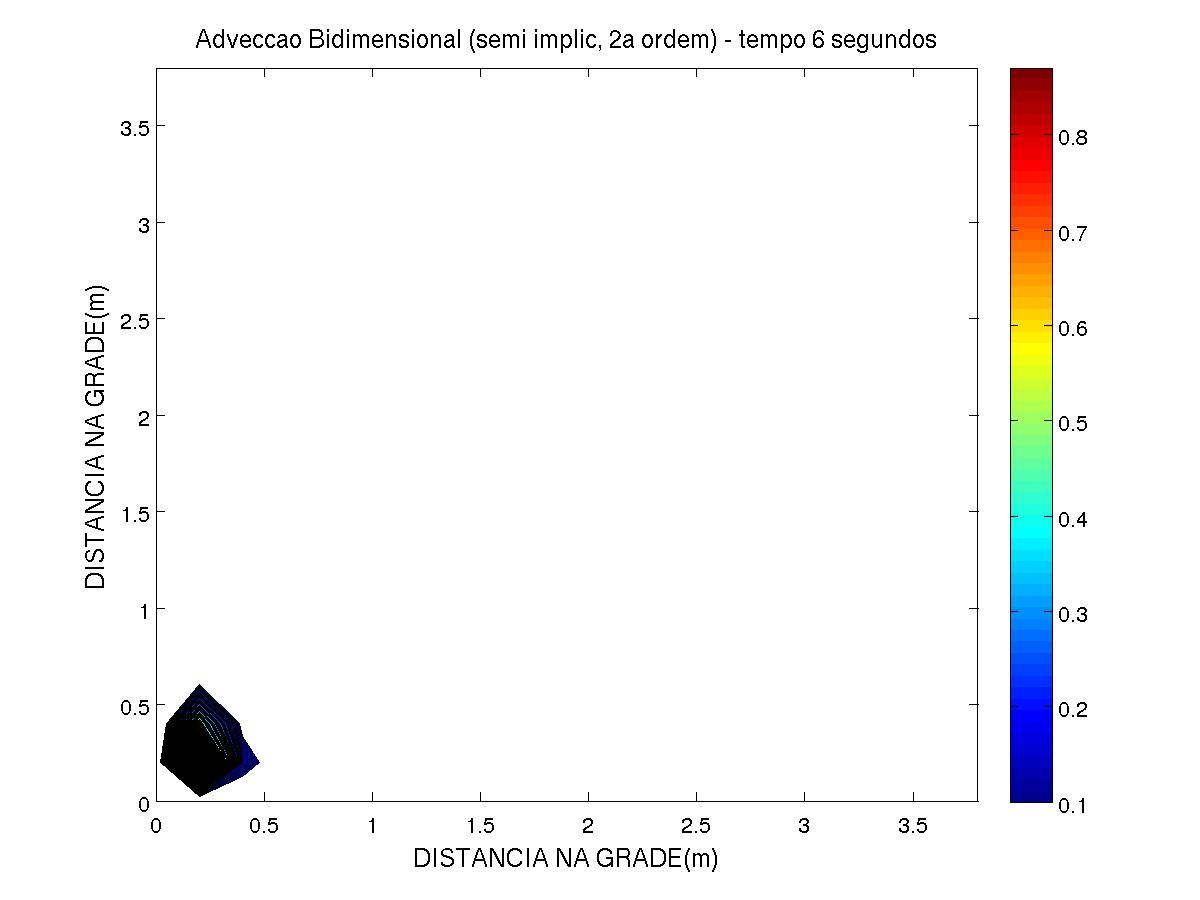
\includegraphics{/home/tparente/danilo/mestrado/github/IOF814/Lista01/outputs/Q02/q02_001.png}
\caption{Fig 1 - Advecção bidimensional de um contaminante teórico, através de discretização com esquema
semi implícito de 2ª ordem. Instante referente ao início da simulação (6 segundos).}
\label{fig2:1}
\end{figure}


\begin{figure}
\centering
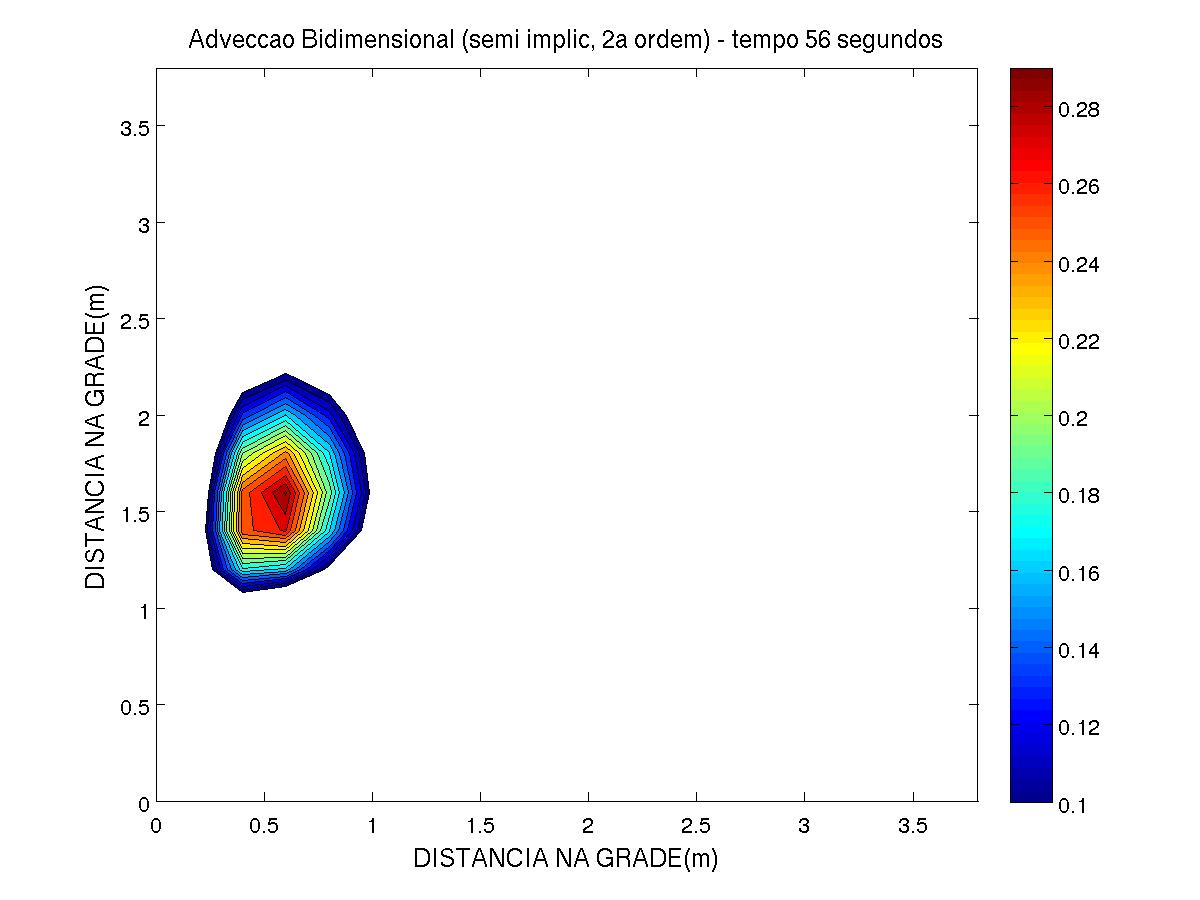
\includegraphics{/home/tparente/danilo/mestrado/github/IOF814/Lista01/outputs/Q02/q02_011.png}
\caption{Fig 2 - Idem a \protect Fig~\ref{fig2:1}, mas para o instante de 56 segundos simulados.}
\label{fig2:2}
\end{figure}

\begin{figure}
\centering
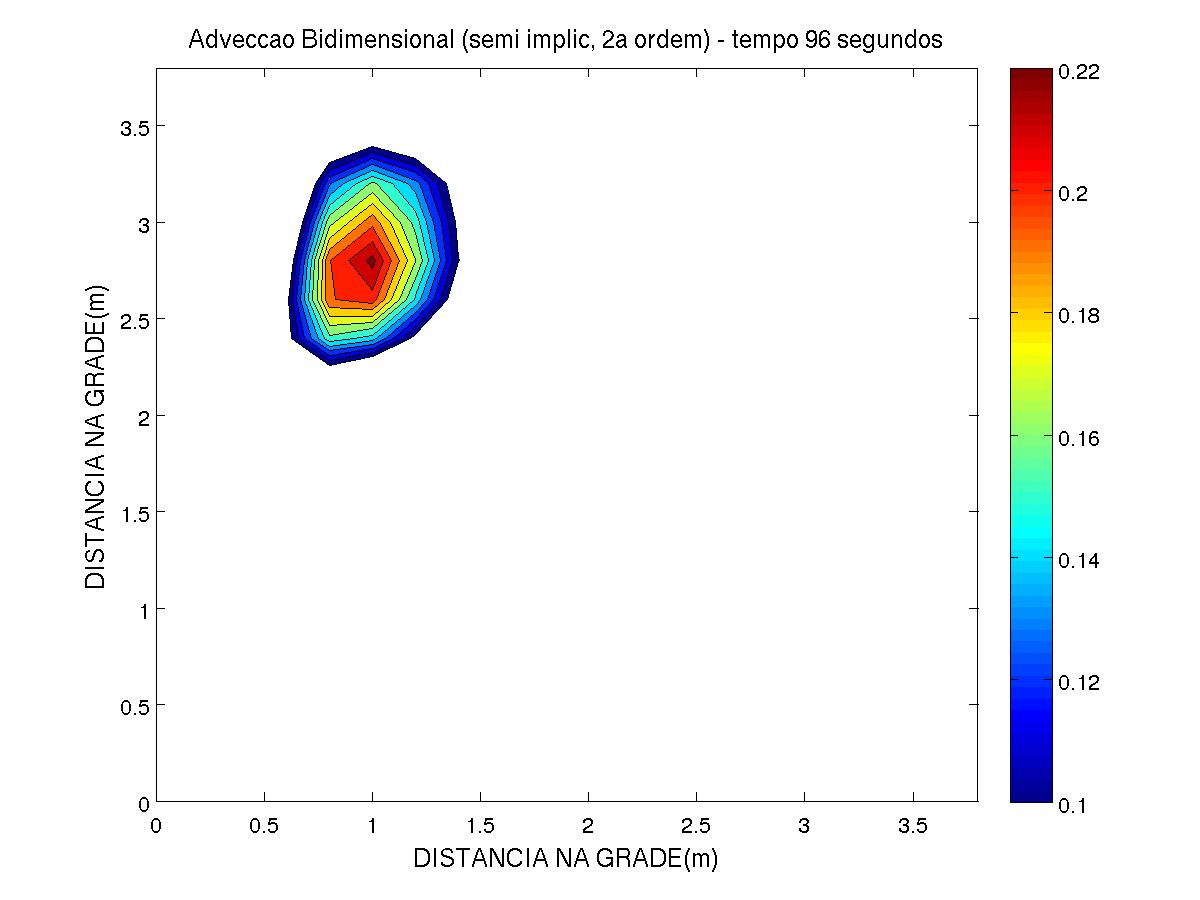
\includegraphics{/home/tparente/danilo/mestrado/github/IOF814/Lista01/outputs/Q02/q02_019.png}
\caption{Fig 3 - Idem a \protect Fig~\ref{fig2:1}, mas para o instante de 96 segundos simulados, referente ao final da
simulação.}
\label{fig2:3}
\end{figure}

    \subparagraph{Q.03 - O que são condições de contorno nas formas não
gradiente, extrapolação linear e radiacional ? Dê exemplos para a
equação da difusão uni-dimensional linear. Que consequências e que
restrições deve ser consideradas ao usar estas condições de contorno
?}

Como não podemos aplicar a fórmula de recorrência ao último ponto de
grade, é necessário impor uma condição de contorno adicional, chamada de
\emph{"Condição de Contorno Computacional"}. Essa condição adicional é
necessária junto a condição inicial e a condição de contorno no primeiro
ponto da grade e é dada em \(f^{n+1}_{j=jmax}\).



\textbf{Condição não Gradiente}

Utiliza-se o valor do penúltimo ponto de grade calculado e repete-se no
último ponto, na seguinte forma:

\begin{equation}
    f^{n+1}_{jmax} = f^{n+1}_{jmax-1}
\end{equation}

Para a equação da difusão unidimensional linear, podemos determinar a
condição de contorno computacional como sendo:

\begin{equation}
    \frac{\partial{f}}{\partial{t}} = D\frac{\partial^2{f}}{\partial{x^2}} \longrightarrow \frac{f^{n+1}_{j} - f^{n}_{j}}{\Delta{t}} = D\bigg( \frac{f^{n}_{j+1} -2f^{n}_{j} + f^{n}_{j-1}}{\Delta{x^2}} \bigg)
    \label{ex3:nGradAdv}
\end{equation}

Desta forma, de (\ref{ex3:nGradAdv}) determinado a fórmula de
recorrência:

\begin{equation}
    f^{n+1}_{j} = f^{n}_{j} + D\frac{\Delta{t}}{\Delta{x^2}}\bigg( f^{n}_{j+1} -2f^{n}_{j} + f^{n}_{j-1} \bigg)
    \label{ex3:nGradAdv_recorrencia}
\end{equation}

Por fim, de (\ref{ex3:nGradAdv_recorrencia}) determinamos o valor no
último ponto de grade da equação da advecção unidimensional linear, na
forma matricial, como:

\begin{equation}
    fren(jmax) = fatu(jmax-1) + D\frac{\Delta{t}}{\Delta{x^2}}\biggr[fatu(jmax) -2fatu(jmax-1) +fatu(jmax-2) \biggr]
\end{equation}

Embora de fácil implementação e não possuir restrição de aplicação, essa
condição conduz a instabilidade do modelo, ao refletir parcialmente o
sinal no contorno, com amplitude igual a
\(A_0tan\bigg( \frac{K\Delta{x}}{2} \bigg)\), ou seja, para
\(K\Delta{x} \longrightarrow 0\) a reflexão tende a zero.

\textbf{Extrapolação Linear}

Utiliza-se os valores dos pontos imediatamente internos ao contorno no
nível de tempo (n). Um exemplo tomando dois pontos é descrito da
seguinte forma:

\begin{equation}
    f^{n+1}_{jmax} = 2f^{n}_{jmax-1} - f^{n}_{jmax-2}
    \label{ex3:extrap}
\end{equation}

onde utiliza-se o penúltimo e antepenúltimo ponto de grade do instante
de tempo atual (n), para se calcular o instante renovado (n+1). Na forma
matricial, (\ref{ex3:extrap}) toma a seguinte forma:

\begin{equation}
    fren(jmax) = 2fatu(jmax-1) - fatu(jmax-2)
\end{equation}

Entretanto, a utilização desta condição de contorno instabilidade o
modelo, mas pode-se reduzir a instabilidade ao adotar mais pontos de
grades. A reflexão na borda, nesta condição de contorno, possui
amplitude \(A_0tan^2\bigg( \frac{K\Delta{x}}{2} \bigg)\), desde que
\(\bigg| tan\bigg( \frac{K\Delta{x}}{2} \bigg) \bigg| < 1\), essa
solução será melhor que a condição não gradiente.

\textbf{Condição Radiacional}

Consiste na advecção de variáveis próximas ao contorno, através de uma
equação de advecção adicional:

\begin{equation}
    \frac{\partial{f}}{\partial{t}} + c_p\frac{\partial{f}}{\partial{x}} = 0
    \label{ex3:radic1}
\end{equation}

Onde o parâmetro \(c_p\) é calculado utilizando-se o penúltimo ponto de
grade (jmax-1) e, então, emprega-se a equação (\ref{ex3:radic1}) para
determinar os valores no contorno (jmax). Usando como exemplo a equação
da difusão uni-dimensional, podemos discretizar (\ref{ex3:radic1}) da
seguinte forma:

\begin{equation}
    \frac{f^{n}_{jmax-1} - f^{n-1}_{jmax-1}}{\Delta{t}} + c_p\frac{f^{n-1}_{jmax-1} - f^{n-1}_{jmax-2}}{\Delta{x}} = 0
    \label{ex3:radic2}
\end{equation}

E, isolando \(c_p\), obtemos, para o penúltimo ponto de grade, a
seguinte equação:

\begin{equation}
    c_p = -\frac{ \frac{f^{n}_{jmax-1} - f^{n-1}_{jmax-1}}{\Delta{t}} }{ \frac{f^{n-1}_{jmax-1} - f^{n-1}_{jmax-2}}{\Delta{x}} }
    \label{ex3:radic3}
\end{equation}

Desta maneira, tendo \(c_p\) calculado, podemos aplicar a condição de
contorno radiacional para o último ponto de grade de um modelo para a
equação da difusão 1D da seguinte forma:

\begin{equation}
    fren(jmax)=fatu(jmax) - cp*\frac{\Delta{t}}{\Delta{x}}*(fatu(jmax) - fatu(jmax-1));
\end{equation}

Importante notar que, independente da equação sendo modelada, o
distúrbio será propagado para o contorno utilizando uma equação de
advecção aplicada no contorno e nas proximidades dele. A qualidade desta
condição é dada, portanto, pela tendência do distúrbio ser
eficientemente advectado para fora do domínio.

\textbf{Conclusão}

Por fim, as melhores condições de contorno são as que provocam mínima
reflexão do sinal nas bordas e mantém a continuidade dos resultados
próximo aos limites da grade.

    \subparagraph{Q.04 - Implemente dois modelos de advecção de um sinal
retangular numa grande uni-dimensional, através de esquemas avançados no
tempo, que utilizam diferenças finitas no espaço de 1ª ordem e de 4ª
ordem. Compare os resultados dos dois
modelos.}\label{q.04---implemente-dois-modelos-de-advecuxe7uxe3o-de-um-sinal-retangular-numa-grande-uni-dimensional-atravuxe9s-de-esquemas-avanuxe7ados-no-tempo-que-utilizam-diferenuxe7as-finitas-no-espauxe7o-de-1uxaa-ordem-e-de-4uxaa-ordem.-compare-os-resultados-dos-dois-modelos.}

A equação da advecção é dada por:

\begin{equation}
    \frac{\partial{f}}{\partial{t}} + c\frac{\partial{f}}{\partial{x}} = 0
    \label{ex4:1}
\end{equation}

Discretizando (\ref{ex4:1}) para o esquema avançado no tempo e retardado
no espaço de \textbf{1ª ordem}, teremos:

\begin{equation}
    \frac{f^{n+1}_{j} - f^{n-1}_{j}}{\Delta{t}} + c\Biggl( \frac{f^{n}_{j} - f^{n}_{j-1}}{\Delta{x}} \Biggl) = 0
    \label{ex4:2}
\end{equation}

A fórmula de recorrência será então:

\begin{equation}
    f^{n+1}_{j} = f^{n}_{j} - c\frac{\Delta{t}}{\Delta{t}}(f^{n}_{j} - f^{n}_{j-1})
    \label{ex4:3}
\end{equation}

E, na forma matricial, (\ref{ex4:3}) ficará:

\begin{equation}
fren(2:jmax-1) = fatu(2:jmax-1) - c\frac{dt}{dx}\biggr[ fatu(2:jmax-1) - fatu(1:jmax-2) \biggr]
\label{ex4:4}
\end{equation}

onde fren representa o nível de tempo renovado (n+1) e fatu o nível de
tempo atual (n).

Discretizando (\ref{ex4:1}), para o mesmo esquema, mas desta vez de
\textbf{4ª ordem}, é necessário trabalhar de forma diferente. Sendo
assim, desenvolvemos inicialmente a discretização no esquema avançado no
tempo:

\begin{equation}
    \frac{\partial{f}}{\partial{t}} = \frac{f^{n+1}_{j} - f^{n}_{j}}{\Delta{t}}
    \label{ex4:5}
\end{equation}

Já para o esquema de 4ª ordem no espaço, teremos um conjunto de 5
equações:

Uma geral, em que os pontos de grade calculados são de 3:jmax-2,
pensando em um aplicação no matlab, onde jmax é o a quantidade máxima de
pontos em j:

\begin{equation}
    \frac{\partial{f}}{\partial{x}} = \frac{\biggl( f^{n}_{j-2} - 8f^{n}_{j-1} + 8f^{n}_{j+1} - f^{n}_{j+2}
    \bigg)}{12\Delta{x}}
    \label{ex4:6}
\end{equation}

Para, respectivamente, o 1º, 2º, penúltimo e último ponto de grade,
teremos as seguintes equações:

\begin{equation}
\begin{cases}
    \frac{\partial{f}}{\partial{x}} = \frac{\biggl( - 25f^{n}_{j} + 48f^{n}_{j+1} - 36f^{n}_{j+2} + 16f^{n}_{j+3} - 3f^{n}_{j+4} \bigg)}{12\Delta{x}} & \text{(A)}\\
    \frac{\partial{f}}{\partial{x}} = \frac{\biggl( - 3f^{n}_{j-1} - 10f^{n}_{j} + 18f^{n}_{j+1} - 6f^{n}_{j+2} + f^{n}_{j+3} \bigg)}{12\Delta{x}} & \text{(B)}\\
    \frac{\partial{f}}{\partial{x}} = \frac{\biggl( - f^{n}_{j-3} + 6f^{n}_{j-2} - 18f^{n}_{j-1} + 10f^{n}_{j} + 3f^{n}_{j+1} \bigg)}{12\Delta{x}} & \text{(C)}\\
    \frac{\partial{f}}{\partial{x}} = \frac{\biggl( 3f^{n}_{j-4} - 16f^{n}_{j-3} + 36f^{n}_{j-2} - 48f^{n}_{j-1} + 25f^{n}_{j} \bigg)}{12\Delta{x}} & \text{(D)}
    \label{ex4:7}
\end{cases}
\end{equation}

Sendo assim, ao programarmos um modelo com a equação de advecção
discretiza avançada no tempo e de 4ª ordem no espaço, teremos o seguinte
conjunto de equações a ser implementado.

Iniciamos o desenvolvimento da discretização de (\ref{ex4:1}) pelo caso
mais geral, equações (\ref{ex4:5}) e (\ref{ex4:6}):

\begin{equation}
    \frac{f^{n+1}_{j} - f^{n}_{j}}{\Delta{t}} + \frac{c}{12\Delta{x}}\biggl( f^{n}_{j-2} - 8f^{n}_{j-1} + 8f^{n}_{j+1} - f^{n}_{j+2} \bigg) = 0
    \label{ex4:8}
\end{equation}

Que, isolando \(f^{n+1}_{j}\) obtemos a função de renovação:

\begin{equation}
    f^{n+1}_{j} = f^{n}_{j}-c\frac{\Delta{t}}{12\Delta{x}}\biggl( f^{n}_{j-2} - 8f^{n}_{j-1} + 8f^{n}_{j+1} - f^{n}_{j+2} \bigg)
    \label{ex4:9}
\end{equation}

De forma análoga, podemos reescrever o conjunto de equações
(\ref{ex4:7}), isolando o nível renovado de tempo:

\begin{equation}
    \begin{cases}
            f^{n+1}_{j} = f^{n}_{j}-c\frac{\Delta{t}}{12\Delta{x}}\biggl( - 25f^{n}_{j} + 48f^{n}_{j+1} - 36f^{n}_{j+2} + 16f^{n}_{j+3} - 3f^{n}_{j+4} \bigg) & (A) \\
            f^{n+1}_{j} = f^{n}_{j}-c\frac{\Delta{t}}{12\Delta{x}}\biggl( - 3f^{n}_{j-1} - 10f^{n}_{j} + 18f^{n}_{j+1} - 6f^{n}_{j+2} + f^{n}_{j+3}  \bigg) & (B) \\
            f^{n+1}_{j} = f^{n}_{j}-c\frac{\Delta{t}}{12\Delta{x}}\biggl( - f^{n}_{j-3} + 6f^{n}_{j-2} - 18f^{n}_{j-1} + 10f^{n}_{j} + 3f^{n}_{j+1} \bigg) & (C) \\
            f^{n+1}_{j} = f^{n}_{j}-c\frac{\Delta{t}}{12\Delta{x}}\biggl( 3f^{n}_{j-4} - 16f^{n}_{j-3} + 36f^{n}_{j-2} - 48f^{n}_{j-1} + 25f^{n}_{j} \bigg) & (D)
            \label{ex4:10}
    \end{cases}
\end{equation}

A solução numérica de ambos os esquemas de discretização é realizada no
arquivo lista1\_Q04\_ord01.m e lista1\_Q04\_ord04.m, a seguir, seguem os
resultados obtidos nos modelos elaborados.

Comparativamente, nota-se que o esquema de ordem 4 (Fig~\ref{fig4:2}) possui uma
instabilidade maior que o esquema de ordem 1 (Fig~\ref{fig4:1}), com ruídos que
interferem no sinal e, com o tempo, amplificam-se. Desta forma, o
esquema de baixa ordem foi considerado o mais adequado para modelar a
advecção do sinal retangular do exercício.

Adicionalmente, foram estimados, utilizando-se as próprias rotinas do
Matlab, o tempo de processamento de cada modelo, onde o modelo de ordem
1 rodou em, aproximadamente, 6 segundos o dobro de domínio temporal que
o esquema de ordem 4 rodou em 4 segundos. Apesar o tempo menor do
segundo esquema, conclui-se que, em questão de custo computacional e
eficiência de processamento, o esquema de ordem 1 (baixa ordem) é o
melhor para a questão. Ainda, comparando os passos de tempo de cada
modelo, o esquema de baixa ordem rodou, de forma estável, com um
\(\Delta{t}\) 10 vezes maior que o utilizado no esquema de alta ordem
que, com \(\Delta{t} > 1\) instabilizou rapidamente.

\begin{figure}
\centering
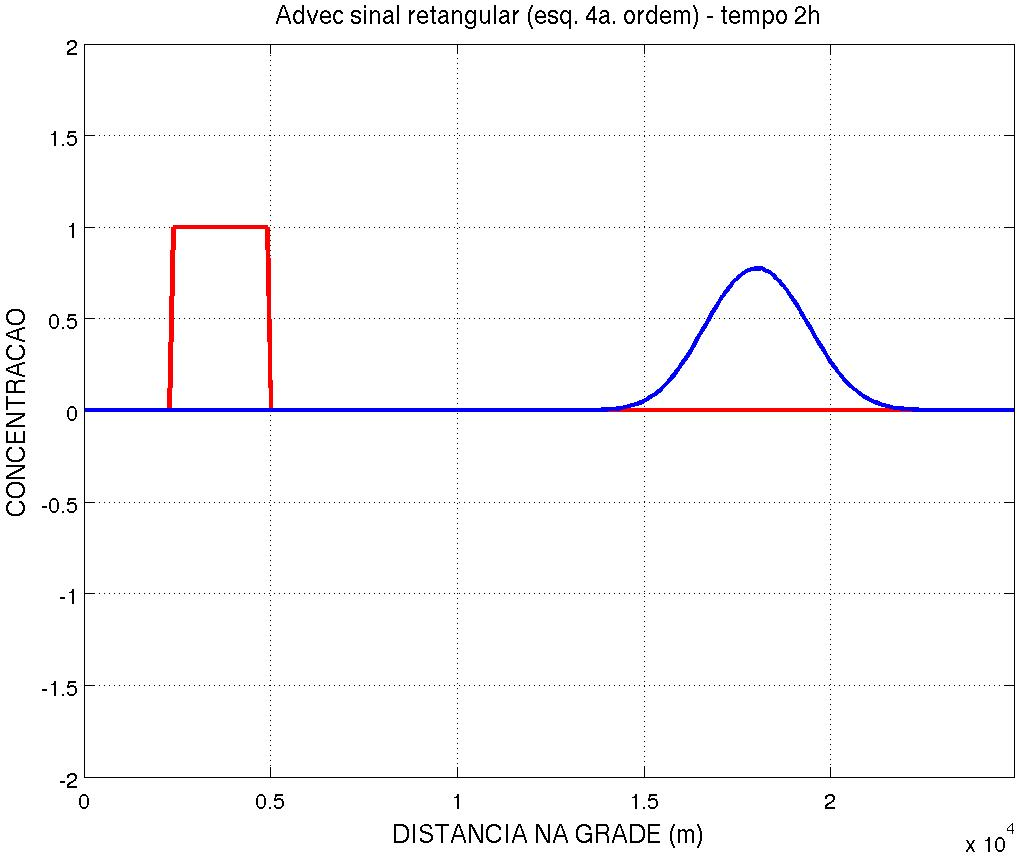
\includegraphics{/home/tparente/danilo/mestrado/github/IOF814/Lista01/outputs/Q04_ord01/q04_ord01_7200.png}
\caption{Fig 4 - Advecção de um sinal retangular em esquema avançado no tempo e retardado no espaço de 1ª ordem.}
\label{fig4:1}
\end{figure}

\begin{figure}
\centering
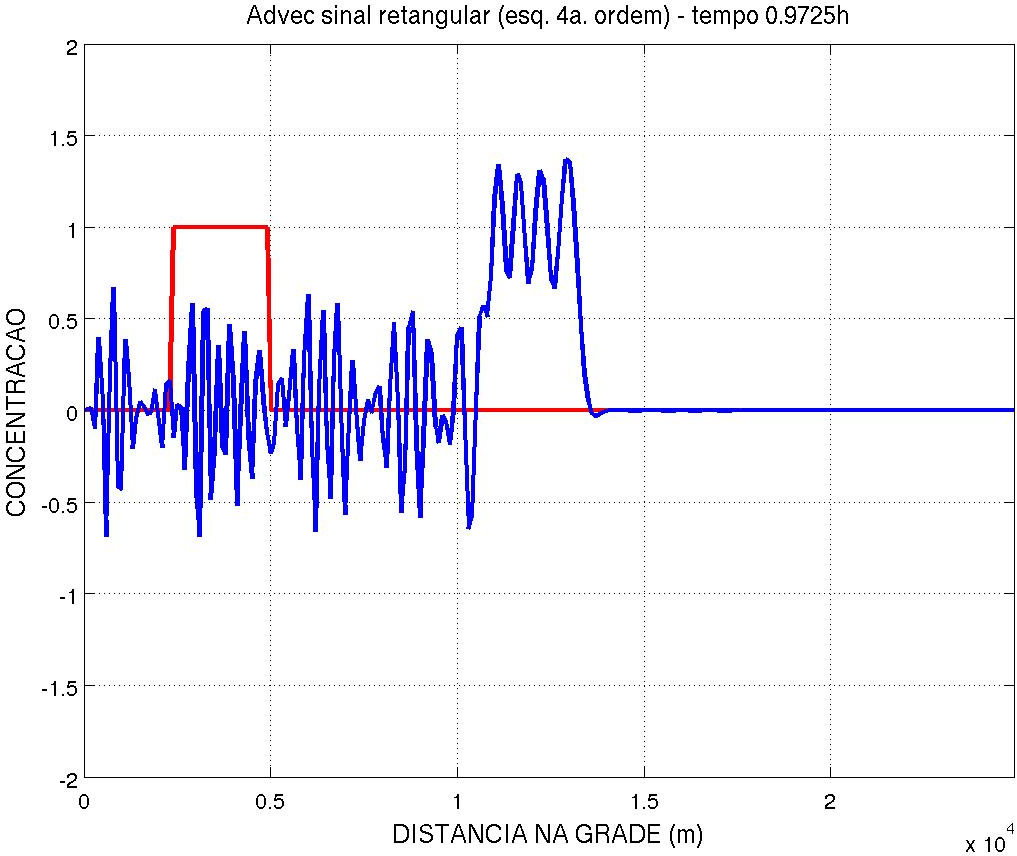
\includegraphics{/home/tparente/danilo/mestrado/github/IOF814/Lista01/outputs/Q04_ord04/q04_ord04_3501.png}
  \caption{Fig 5 - Advecção de um sinal retangular em esquema avançado no tempo e retardado no espaço de 4ª ordem.}
\label{fig4:2}
\end{figure}

    \subparagraph{Q.05 - Determine os coeficientes da forma discretiza da
equação da
difusão}
\begin{equation}
    \frac{\partial{f}}{\partial{t}} - D\frac{\partial^2{f}}{\partial{x^2}} = \alpha f^{n+1}_{j} + \beta f^{n}_{j+1} + \gamma f^{n}_{j-1} + \delta f^{n-1}_{j}
    \label{ex5:1}
\end{equation}

\subparagraph{a partir de expressões da Série de Taylor. Qual é a
principal utilidade do "Método dos coeficientes
indefinidos"?}

Inicialmente expandimos os termos do lado direito da equação
(\ref{ex5:1}), truncando a expansão no quarto termo, para termos um
sistema fechado adiante (4 equações para 4 coeficientes):

\begin{equation}
\begin{aligned}
    f^{n+1} = f^{n} + \Delta{t}\frac{\partial{f}}{\partial{t}} + \frac{\Delta{t}^2}{2}\frac{\partial^2{f}}{\partial{t^2}} + \frac{\Delta{t}^3}{3!}\frac{\partial^3{f}}{\partial{t^3}} + ...
    \\
    f^{n-1} = f^{n} - \Delta{t}\frac{\partial{f}}{\partial{t}} + \frac{\Delta{t}^2}{2}\frac{\partial^2{f}}{\partial{t^2}} - \frac{\Delta{t}^3}{3!}\frac{\partial^3{f}}{\partial{t^3}} + ...
    \\
    f_{j+1} = f_{j} + \Delta{x}\frac{\partial{f}}{\partial{x}} + \frac{\Delta{t}^2}{2}\frac{\partial^2{f}}{\partial{x^2}} + \frac{\Delta{t}^3}{3!}\frac{\partial^3{f}}{\partial{x^3}} + ...
    \\
    f_{j-1} = f_{j} - \Delta{x}\frac{\partial{f}}{\partial{x}} + \frac{\Delta{t}^2}{2}\frac{\partial^2{f}}{\partial{x^2}} - \frac{\Delta{t}^3}{3!}\frac{\partial^3{f}}{\partial{x^3}} + ...
\end{aligned}
    \label{ex5:2}
\end{equation}

Aplicando o conjunto de equações (\ref{ex5:2}) em (\ref{ex5:1}),
obteremos:

\begin{equation}
\begin{aligned}
    \frac{\partial{f}}{\partial{t}} - D\frac{\partial^2{f}}{\partial{x^2}} =
    \alpha (f^{n} + \Delta{t}\frac{\partial{f}}{\partial{t}} + \frac{\Delta{t}^2}{2}\frac{\partial^2{f}}{\partial{t^2}}+ \frac{\Delta{t}^3}{3!}\frac{\partial^3{f}}{\partial{t^3}}) +  \\
    \beta (f_{j} + \Delta{x}\frac{\partial{f}}{\partial{x}} + \frac{\Delta{t}^2}{2}\frac{\partial^2{f}}{\partial{x^2}}- \frac{\Delta{t}^3}{3!}\frac{\partial^3{f}}{\partial{x^3}}) +
    \gamma (f^{n} - \Delta{t}\frac{\partial{f}}{\partial{t}} + \\ + \frac{\Delta{t}^2}{2}\frac{\partial^2{f}}{\partial{t^2}}+ \frac{\Delta{t}^3}{3!}\frac{\partial^3{f}}{\partial{t^3}}) +
    \delta (f_{j} - \Delta{x}\frac{\partial{f}}{\partial{x}} + \frac{\Delta{t}^2}{2}\frac{\partial^2{f}}{\partial{x^2}}- \frac{\Delta{t}^3}{3!}\frac{\partial^3{f}}{\partial{x^3}})
\end{aligned}
    \label{ex5:3}
\end{equation}

Associando os termos do lado direito aos termos do lado esquerdo de
(\ref{ex5:3}), obteremos o seguinte sistema de equações:

\begin{equation}
  \begin{cases}
    \alpha + \beta + \gamma + \delta = 0 & \text{(a)}\\
    \alpha \Delta{t} - \delta \Delta{t} = 0  & \text{(b)} \\
    \beta \Delta{x} - \gamma \Delta{x} = 0 \to \beta = \gamma & \text{(c)}\\
    \beta \frac{\partial{\Delta{x^2}}}{2} + \gamma \frac{\partial{\Delta{x^2}}}{2} = -D \to \beta + \gamma = \frac{-2D}{\Delta{x^2}} & \text{(d)}
  \end{cases}
  \label{ex5:4}
\end{equation}

Para determinar os coeficientes \(\alpha\), \(\beta\), \(\gamma\) e
\(\delta\), precisamos resolver o sistema de equações (\ref{ex5:4}).

\textbf{Determinando \(\alpha\)}

Multiplica-se (4.a) por \(\Delta{t}\) e soma-se (4.b):

\begin{equation}
    (\alpha + \beta + \gamma + \delta)\Delta{t} + \alpha \Delta{t} - \gamma \Delta{t} = 0 \to 2\alpha{\Delta{t}} + \beta{\Delta{t}} + \gamma{\Delta{t}} = 0 \\
    \therefore 2\alpha + \beta + \gamma = \frac{1}{\Delta{t}}
    \label{ex5:5}
\end{equation}

Multiplicando (\ref{ex5:4}.d) por (-1) e somando (\ref{ex5:4}), obtemos:

\begin{equation}
    \alpha = \frac{1}{2\Delta{t}} + \frac{D}{\Delta{x^2}}
    \label{ex5:6}
\end{equation}

\textbf{Determinando \(\delta\)}

Aplica-se (\ref{ex5:6}) em (\ref{ex5:4}.b):

\begin{equation}
    \begin{aligned}
        (\frac{1}{2\Delta{t}} + \frac{D}{\Delta{x^2}})\Delta{t} - \delta \Delta{t} = 0 \to  \frac{1}{2} + \frac{\Delta{t}D}{\Delta{x^2}} - \delta{\Delta{t}} = 1 \to \delta = -\frac{1}{\Delta{t}} + \frac{D}{\Delta{x^2}}
    \end{aligned}
    \label{ex5:7}
\end{equation}

\textbf{Determinando \(\beta\)}

Aplicando (\ref{ex5:4}.c) em (\ref{ex5:4}.d):

\begin{equation}
    \begin{aligned}
        \beta{\frac{\Delta{x^2}}{2}} + \beta{\frac{\Delta{x^2}}{2}} = -D \to \beta{\Delta{x^2}} = -D \\
        \therefore \beta = -\frac{D}{\Delta{x^2}}
    \end{aligned}
    \label{ex5:8}
\end{equation}

\textbf{Determinando \(\gamma\)}

Como de (\ref{ex5:4}.c) \(\beta = \gamma\), então:

\begin{equation}
    \gamma = -\frac{D}{\Delta{x^2}}
    \label{ex5:9}
\end{equation}

Finalmente, aplicamos as equações (\ref{ex5:6}) a (\ref{ex5:9}) em
(\ref{ex5:1}) e obteremos:

\begin{equation}
\frac{\partial{f}}{\partial{t}} - D\frac{\partial^2{f}}{\partial{x^2}} =
    (\frac{1}{2\Delta{t}} + \frac{D}{\Delta{x^2}})f^{n+1}_{j} +
    (-\frac{D}{\Delta{x^2}})f^{n}_{j+1} +
    (-\frac{D}{\Delta{x^2}})f^{n}_{j-1} +
    (-\frac{1}{2\Delta{t}} + \frac{D}{\Delta{x^2}})f^{n-1}_{j}
    \label{ex5:10}
\end{equation}

Desenvolvendo a equação (\ref{ex5:10}), obteremos:

\begin{equation}
    \frac{\partial{f}}{\partial{t}} - D\frac{\partial^2{f}}{\partial{x^2}} =
    \frac{f^{n+1}_{j}}{2\Delta{t}} + \frac{Df^{n+1}_{j}}{\Delta{x^2}} -
    \frac{Df^{n}_{j+1}}{\Delta{x^2}} - \frac{Df^{n}_{j-1}}{\Delta{x^2}} -
    \frac{f^{n-1}_{j}}{2\Delta{t}} + \frac{Df^{n-1}_{j}}{\Delta{x^2}}
    \label{ex5:11}
\end{equation}

Reorganizando a equação (\ref{ex5:11}), finalmente obtemos a equação da
difusão discretizada com esquema centrado no tempo e no espaço
pseudo-implícito:

\begin{equation}
    \frac{f^{n+1}_{j} - f^{n-1}_{j}}{2\Delta{t}} =
    \frac{D}{\Delta{x^2}}(f^{n}_{j+1} + f^{n}_{j-1} - f^{n+1}_{j} - f^{n-1}_{j})
    \label{ex5:12}
\end{equation}

A principal utilidade de se utilizar o \textbf{"Método dos coeficientes
indefinidos"} é que podemos usar mais pontos no esquema de
discretização. Neste caso, foram utilizados 4 pontos e, portanto, 4
coeficientes foram definidos. Em caso de de usar 6, 8, 10 pontos,
poderíamos ter, respectivamente, 6, 8 ou 10 coeficientes a serem
determinados, sendo um artifício para lidar com a instabilidade do
esquema utilizado na discretização.

    \subparagraph{Q.06 - Implemente um modelo numérico de
advecção-difusão-decaimento 2D para a área costeira ao largo de Santos
(SP), para os limites (46.5ºW - 46.2ºW; 23.95ºS - 24.15ºS). Processe o
modelo para a dispersão de um contaminante despejado de forma contínua
no ponto 46.35ºW 24.01ºS (simulando a operação do emissário submarino) e
a dispersão de um contaminante despejado instantaneamente em 46.35ºW
24.10ºS (simulando acidente com embarcação tem trânsito). Processe o
modelo com correntes de 1m/s para Norte, Nordeste e Noroeste. Forneça
mapas das plumas de contaminantes e detecte que áreas costeiras podem
ser atingidas em cada
caso.}

Fórmula de recorrência:

\begin{equation}
\begin{aligned}
    \frac{f^{n+1}_{j,k} - f^{n}_{j,k}}{\Delta{t}} + \frac{u + |u|}{2}\frac{f^{n}_{j,k} - f^{n}_{j-1,k}}{\Delta{x}} + \frac{u - |u|}{2}\frac{f^{n}_{j+1,k} - f^{n}_{j,k}}{\Delta{x}} + \\
    \frac{v + |v|}{2}\frac{f^{n}_{j,k} - f^{n}_{j,k-1}}{\Delta{y}} + \frac{v - |v|}{2}\frac{f^{n}_{j,k+1} - f^{n}_{j,k}} {\Delta{y}} = \\
    D_x\frac{f^{n}_{j+1,k} - 2f^{n}_{j,k} + f^{n}_{j-1,k}}{\Delta{x^2}} + D_y\frac{f^{n}_{j,k+1} - 2f^{n}_{j,k} + f^{n}{j,k-1}}{\Delta{y^2}} - rf^{n}_{j,k}
\end{aligned}
\end{equation}

O programa elaborado para resolver este exercício está no arquivo
\textbf{Lista1\_Q06.m} e as saídas do modelo estão em \textbf{outputs/}.

Para o cenário com ventos para Norte, notamos que as plumas, tanto do
emissário quanto do acidente com embarcação, evoluem em direção a região
central do domínio modelado, atingindo, eventualmente, a costa
diretamente na praia de Santos. Considerando a velocidade das correntes,
a pluma mais externa não atingirá a costa no período de simulação de 30
minutos, mas aumentando este período a pluma alcançará de fato, embora
com concentrações muito baixas (em geral abaixo de \(10^{-7}\)).

No cenário com ventos para Noroeste, a pluma do emissário atinge a
região da ponta da praia e entrada do Porto de Santos, com elevadas
concentrações. Já a pluma do acidente evolui para o setor superior leste
do domínio, atingindo a região de Guarujá e Bertioga e, por um período
de simulação maior, a pluma atingiria parte do Litoral Norte de São
Paulo.

Por fim, o último cenário modelado, com ventos para Noroeste, a pluma do
emissário a boca do estuário de São Vicente, enquanto que a pluma do
acidente, por sua vez, atinge a região a Leste da grade, alcançando
principalmente a região da Praia Grande e demais regiões. Da mesma forma
que no segundo cenário.

\end{document}
